% !TeX program = xelatex

\documentclass{article}
\usepackage{sarcastikz}
\usepackage{fontspec}
\newfontfamily{\comicfont}{Gloria Hallelujah}
\setmainfont{Roboto}
\usepackage[landscape]{geometry}
\usetikzlibrary{calc,decorations.pathmorphing,patterns, backgrounds, patterns}
%\usepackage[weather]{ifsym}
\usepackage{bbding} 
\newcounter{comiccount}
\stepcounter{comiccount}

\makeatletter

\pgfdeclaredecoration{penciline}{initial}{
	\state{initial}[width=+\pgfdecoratedinputsegmentremainingdistance,auto corner on length=1mm,]{
		\pgfpathcurveto%
		{% From
			\pgfqpoint{\pgfdecoratedinputsegmentremainingdistance}
			{\pgfdecorationsegmentamplitude}
		}
		{%  Control 1
			\pgfmathrand
			\pgfpointadd{\pgfqpoint{\pgfdecoratedinputsegmentremainingdistance}{0pt}}
			{\pgfqpoint{-\pgfdecorationsegmentaspect\pgfdecoratedinputsegmentremainingdistance}%
				{\pgfmathresult\pgfdecorationsegmentamplitude}
			}
		}
		{%TO 
			\pgfpointadd{\pgfpointdecoratedinputsegmentlast}{\pgfpoint{1pt}{1pt}}
		}
	}
	\state{final}{}
}
\makeatother

\newenvironment{comics}{%
	\section*{{\Huge sarcasTikz }- grad school in \LaTeX}%
	\begin{center}%
}
{%

\vspace{3mm}	
\thecomiccount - Adarsh
\end{center}%
\stepcounter{comiccount}
}

\newcommand\newdummy[2][]{\begin{scope}[#2] 
\dummy[#1]
\end{scope}}
% colors
\definecolor{skycolor}{HTML}{87CEFA}
\begin{document}
	

\begin{comics}
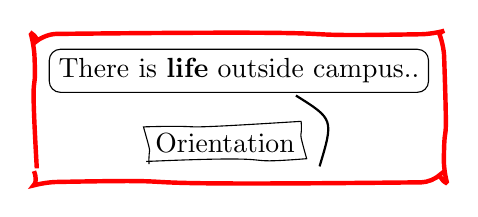
\begin{tikzpicture}[framed, scale=0.6, decoration=penciline, background rectangle/.style={ultra thick,draw=red, rounded corners, decorate}]
\begin{scope}
\node[rectangle,draw, decorate] at (3.5,3.5) {\comicfont Orientation};
\draw[thick] (5.5, 3) .. controls (5.8, 4) .. (5, 4.5);
\node[rectangle, rounded corners, draw] at ([yshift=0.5cm]current bounding box.north) {There is {\bf life} outside campus..};
\end{scope}

\begin{scope}
\dummy[tshirt=black, pant=blue!40!green, shoe, boyhair, viewright, normal]
\end{scope}

\begin{scope}[xshift=4cm]
\dummy[pupil=green, tomhair, hair=brown, tshirt=white, pant=blue, shoe=brown, viewleft, speak]
\end{scope}
\end{tikzpicture}
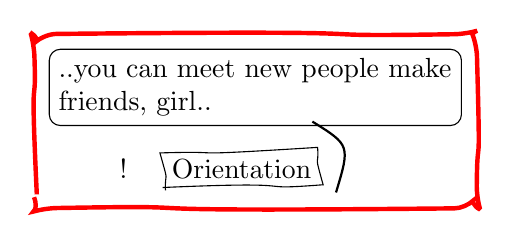
\begin{tikzpicture}[framed, scale=0.6, decoration=penciline, background rectangle/.style={ultra thick,draw=red, rounded corners, decorate}]
\begin{scope}
\node[rectangle,draw, decorate] at (3.5,3.5) {\comicfont Orientation};
\draw[thick] (5.5, 3) .. controls (5.8, 4) .. (5, 4.5);
\node[rectangle, rounded corners, draw, text width = 5cm] at ([yshift=0.7cm]current bounding box.north) {..you can meet new people make friends, girl..};
\node[] at (1,3.5) {!};
\end{scope}

\begin{scope}
\dummy[tshirt=black, pant=blue!40!green, shoe, boyhair, poker]
\end{scope}

\begin{scope}[xshift=4cm]
\dummy[pupil=green, tomhair, hair=brown, tshirt=white, pant=blue, shoe=brown, viewleft, speak]
\end{scope}
\end{tikzpicture}
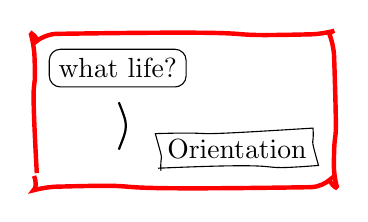
\begin{tikzpicture}[framed, scale=0.6, decoration=penciline, background rectangle/.style={ultra thick,draw=red, rounded corners, decorate}]
\begin{scope}
\node[rectangle,draw, decorate] at (3.5,3.5) {\comicfont Orientation};
\draw[thick] (1, 3.5) .. controls (1.2, 4) .. (1, 4.5);
\node[rectangle, rounded corners, draw] at ([yshift=0.7cm]current bounding box.north west) {what life?};
\end{scope}

\begin{scope}
\dummy[tshirt=black, pant=blue!40!green, shoe, boyhair, viewright, speak]
\end{scope}

\begin{scope}[xshift=4cm]
\dummy[pupil=green, tomhair, hair=brown, tshirt=white, pant=blue, shoe=brown, poker]
\end{scope}
\end{tikzpicture}
\end{comics}

%% Eclipse
\begin{comics}
	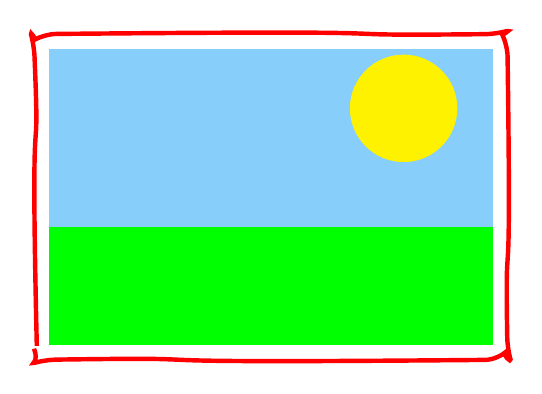
\begin{tikzpicture}[framed, scale=0.75, decoration=penciline, background rectangle/.style={ultra thick,draw=red, rounded corners, decorate}]
	\begin{scope}
	\filldraw[green](-2,0) rectangle (5.5,2);
	\filldraw[skycolor](-2,2) rectangle (5.5,5);
	\filldraw[yellow] (4,4) circle (0.9cm);
	\end{scope}
	
	\begin{scope}
	\dummy[tshirt=black, pant=blue!40!green, shoe, boyhair, normal]
	\end{scope}
	\end{tikzpicture}
	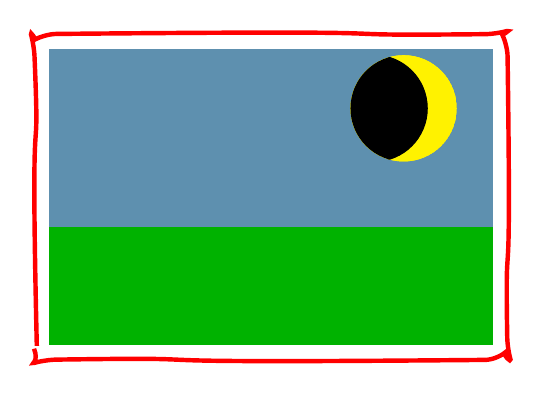
\begin{tikzpicture}[framed, scale=0.75, decoration=penciline, background rectangle/.style={ultra thick,draw=red, rounded corners, decorate}]
	\begin{scope}
	\filldraw[green!70!black](-2,0) rectangle (5.5,2);
	\filldraw[skycolor!70!black](-2,2) rectangle (5.5,5);
	\clip (4,4) circle (0.9cm);
	\filldraw[yellow] (4,4) circle (0.9cm);
	\filldraw[black] (3.5,4) circle (0.9cm);
	\end{scope}
	\newdummy[girlhair, hair=black, body=black!30!brown, paperglass]{xshift=-1.2cm, yshift=2cm,scale=0.8}
	\newdummy[tomhair, hair=brown, paperglass]{xshift=0.8cm, yshift=2cm,scale=0.8}
	\newdummy[tomhair, hair=white, tshirt=red, pant=blue, pupil=yellow, paperglass]{xshift=-2cm}
	\newdummy[paperglass, girlhair, hair=brown!50!black, tshirt=blue, pant=black, pupil=green]{xshift=2cm}
	%\begin{scope}
	\newdummy[tshirt=black, pant=blue!40!green, shoe, boyhair]{}
	%\end{scope}
	\end{tikzpicture}
	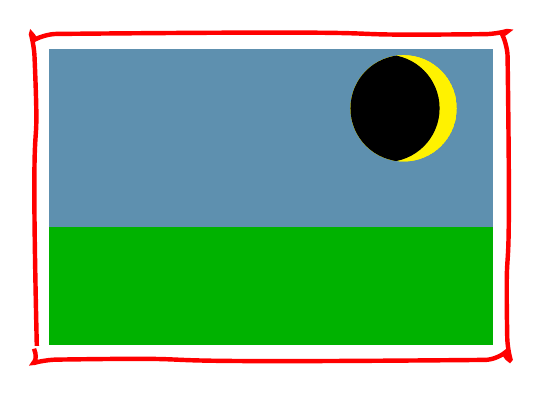
\begin{tikzpicture}[framed, scale=0.75, decoration=penciline, background rectangle/.style={ultra thick,draw=red, rounded corners, decorate}]
	\begin{scope}
	\filldraw[green!70!black](-2,0) rectangle (5.5,2);
	\filldraw[skycolor!70!black](-2,2) rectangle (5.5,5);
	\clip (4,4) circle (0.9cm);
	\filldraw[yellow] (4,4) circle (0.9cm);
	\filldraw[black] (3.7,4) circle (0.9cm);
	\end{scope}
	\newdummy[girlhair, hair=black, body=black!30!brown, paperglass]{xshift=-1.2cm, yshift=2cm,scale=0.8}
	\newdummy[tomhair, hair=brown, paperglass]{xshift=0.8cm, yshift=2cm,scale=0.8}
	\newdummy[tomhair, hair=white, tshirt=red, pant=blue, pupil=yellow, paperglass]{xshift=-2cm}
	\newdummy[paperglass, girlhair, hair=brown!50!black, tshirt=blue, pant=black, pupil=green]{xshift=2cm}
	%\begin{scope}
	\newdummy[tshirt=black, pant=blue!40!green, shoe, boyhair, paperglass, smile]{}
	%\end{scope}
	\end{tikzpicture}
\end{comics}

%% supreme court judgement
\begin{comics}
	
\begin{tikzpicture}
	\node[](a){};
	\node[below] at (a) {\comicfont Meanwhile in India..};
	\end{tikzpicture}
	
	
\begin{tikzpicture}[framed, scale=0.9, decoration=penciline, background rectangle/.style={ultra thick,draw=red, rounded corners, decorate}]
	\begin{scope}
	\node[draw=black, rectangle, decorate, minimum width=2.5cm, text width=2.5cm, rotate=30] at (0, 3.5) {\comicfont Instant Triple Talaq Unconstitutional}; 
	\end{scope}
	\newdummy[judge, shoe=blue!40!black, pupil=green!50!black, lawhammer, judgehair, hair=white, poker]{}
	\end{tikzpicture}
	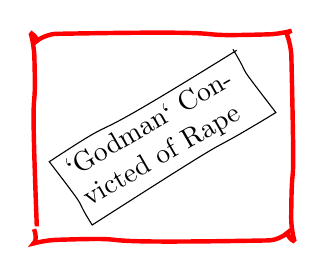
\begin{tikzpicture}[framed, scale=0.9, decoration=penciline, background rectangle/.style={ultra thick,draw=red, rounded corners, decorate}]
	\begin{scope}
	\node[draw=black, rectangle, decorate, minimum width=2.5cm, text width=2.5cm, rotate=30] at (0, 3.5) {\comicfont `Godman` Convicted of Rape}; 
	\end{scope}
	\newdummy[judge, shoe=blue!40!black, pupil=green!50!black, lawhammer, judgehair, hair=white]{}
	\end{tikzpicture}
	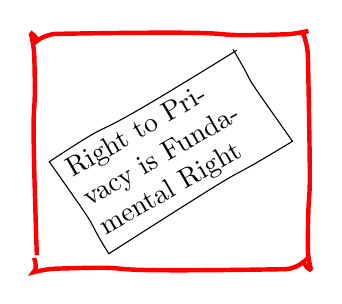
\begin{tikzpicture}[framed, scale=0.9, decoration=penciline, background rectangle/.style={ultra thick,draw=red, rounded corners, decorate}]
	\begin{scope}
	\node[draw=black, rectangle, decorate, minimum width=2.5cm, text width=2.5cm, rotate=30] at (0, 3.5) {\comicfont Right to Privacy is Fundamental Right}; 
	\end{scope}
	\newdummy[judge, shoe=blue!40!black, pupil=green!50!black, lawhammer, judgehair, hair=white, smile]{}
	\end{tikzpicture}
\end{comics}

\pagebreak
%% purdue construction
\begin{comics}
	
\begin{tikzpicture}
	\node[](a){};
	\node[below] at (a) {\comicfont Meanwhile at Purdue..};
	\end{tikzpicture}
	
	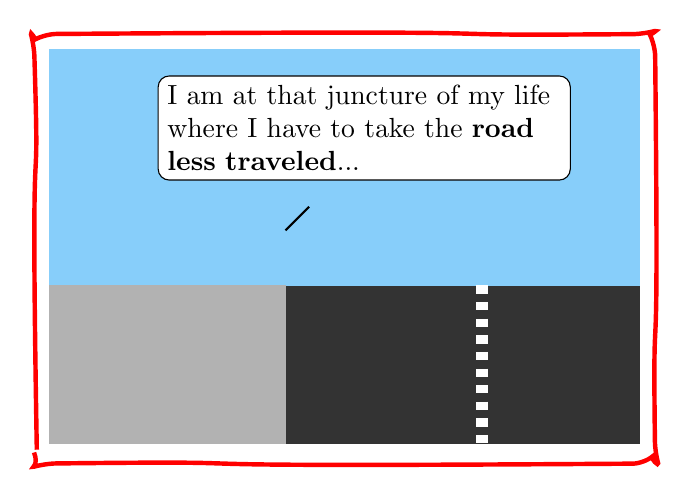
\begin{tikzpicture}[framed, decoration=penciline, background rectangle/.style={ultra thick,draw=red, rounded corners, decorate}]
	\begin{scope}
	\filldraw[white!20!black](-2,0) rectangle (5.5,2);
	\filldraw[skycolor](-2,2) rectangle (5.5,5);
	\draw[dashed, line width=1.5mm, white] (3.5, 2) -- (3.5, 0);
	\filldraw[white!70!black](-2,0) rectangle (1,2);
	\node[rectangle,fill= white, rounded corners, draw, text width=5cm] at (2, 4) {I am at that juncture of my life where I have to take the {\bf road less traveled}...};
	\draw[thick] (1, 2.7) -- (1.3, 3);
	\end{scope}
	
	\begin{scope}
	\newdummy[tshirt=black, pant=blue!40!green, shoe, boyhair, normal]{xshift=-2cm}
	\end{scope}
	\end{tikzpicture}
	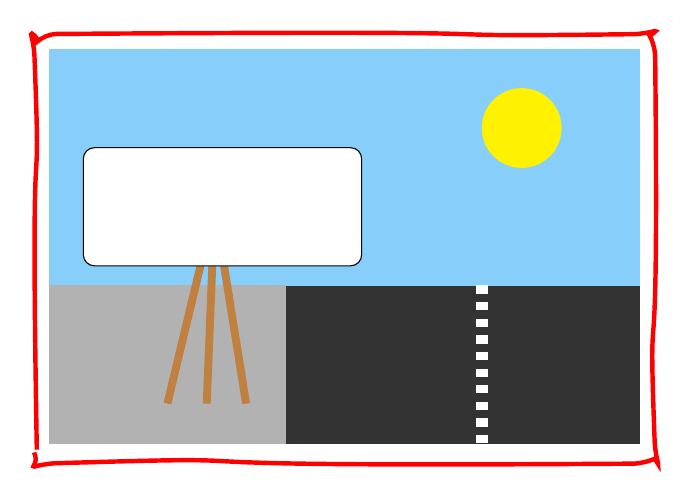
\begin{tikzpicture}[framed, decoration=penciline, background rectangle/.style={ultra thick,draw=red, rounded corners, decorate}]
	\begin{scope}
	\filldraw[white!20!black](-2,0) rectangle (5.5,2);
	\filldraw[skycolor](-2,2) rectangle (5.5,5);
	\filldraw[yellow] (4,4) circle (0.5cm);
	\draw[dashed, line width=1.5mm, white] (3.5, 2) -- (3.5, 0);
	\filldraw[white!70!black](-2,0) rectangle (1,2);
	\draw[brown, line width=1mm] (-0.5, 0.5) -- (0.1, 3) -- (0.5, 0.5);
	\draw[brown, line width=1mm] (0.1, 3) -- (0, 0.5);
	\node[rectangle,fill= orange!70!red, white, rounded corners, draw=black, text width=3.3cm, minimum height=1.5cm] at (0.2, 3) {\bf Construction Ahead. \phantom{aa}$\leftarrow$ DETOUR};
	\end{scope}
	\end{tikzpicture}
\end{comics}

\pagebreak
%% purdue bus
\begin{comics}
	\begin{tikzpicture}
	%\node[](a){};
	%\node[below] at (a) {\comicfont Meanwhile at Purdue..};
	\end{tikzpicture}
	
	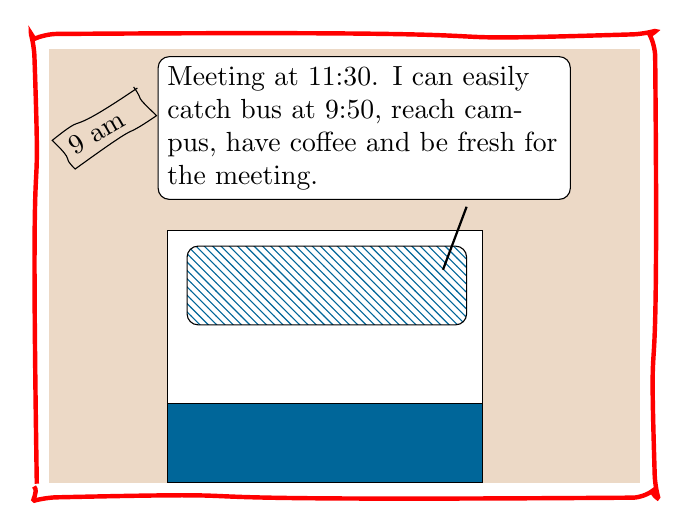
\begin{tikzpicture}[framed, decoration=penciline, background rectangle/.style={ultra thick,draw=red, rounded corners, decorate}]
	\begin{scope}
	\filldraw[brown!30!white](-2,0) rectangle (5.5,5.5);
	\filldraw[white, draw=black](-0.5,0) rectangle (3.5,3.2);
	\filldraw[pattern=north west lines, pattern color=blue!60!green, rounded corners](-0.25,2) rectangle (3.3,3);
	%\draw[dashed, line width=1.5mm, white] (3.5, 2) -- (3.5, 0);
	%\filldraw[white!70!black](-2,0) rectangle (1,2);
	\node[rectangle,fill= white, rounded corners, draw, text width=5cm] at (2, 4.5) {Meeting at 11:30. I can easily catch bus at 9:50, reach campus, have coffee and be fresh for the meeting.};
	\draw[thick] (3, 2.7) -- (3.3, 3.5);
	\node[draw=black, rectangle, decorate, minimum width=1cm, text width=1cm, rotate=30] at (-1.3, 4.5) {\comicfont 9 am}; 
	\end{scope}
	
	\begin{scope}
	\newdummy[tshirt=white, pant=black, boyhair, speak]{}
	\end{scope}
	
	\begin{scope}
	\filldraw[blue!60!green, draw=black](-0.5,0) rectangle (3.5,1);
	\end{scope}
	\end{tikzpicture}
	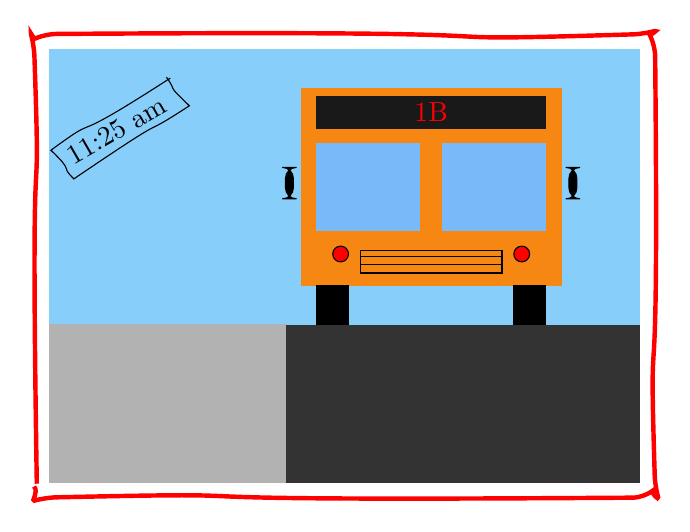
\begin{tikzpicture}[framed, decoration=penciline, background rectangle/.style={ultra thick,draw=red, rounded corners, decorate}]
	\begin{scope}
	\filldraw[white!20!black](-2,0) rectangle (5.5,3.5);
	\filldraw[skycolor](-2,2) rectangle (5.5,5.5);
	%\draw[dashed, line width=1.5mm, white] (3.5, 2) -- (3.5, 0);
	% bus
	\filldraw[yellow!50!red](1.2,2.5) rectangle (4.5,5);
	% mirrors
	\filldraw[black, rounded corners](1.1,4) rectangle (1,3.6);
	\filldraw[black, rounded corners](4.6,4) rectangle (4.7,3.6);
	% 1b pad
	\filldraw[black!90!white](1.4,4.5) rectangle (4.3,4.9);
	\node[color=red] at (2.85, 4.7) {1B};
	% windows
	\filldraw[skycolor!90!blue](1.4,3.2) rectangle (2.7,4.3);
	\filldraw[skycolor!90!blue](3,3.2) rectangle (4.3,4.3);
	% headlights
	\filldraw[red, draw=black] (1.7,2.9) circle (0.1cm);
	\filldraw[red, draw=black] (4,2.9) circle (0.1cm);
	% front bus
	\filldraw[pattern=horizontal lines, pattern color=black](1.95,2.65) rectangle (3.75,2.95);
	\filldraw[black](1.4,2.5) rectangle (1.8,2);
	\filldraw[black](3.9,2.5) rectangle (4.3,2);
	\filldraw[white!70!black](-2,0) rectangle (1,2);
	\node[draw=black, rectangle, decorate, minimum width=1cm, text width=1.5cm, rotate=30] at (-1.1, 4.5) {\comicfont 11:25 am}; 
	\end{scope}
	
	\begin{scope}
	\newdummy[tshirt=white, pant=black, boyhair, angry, viewright, shoe]{xshift=-2cm}
	\end{scope}
	\end{tikzpicture}
\end{comics}


%% winter
%\begin{comics}
%	Work In Progress
%	
%	\begin{tikzpicture}[framed, decoration=penciline, background rectangle/.style={ultra thick,draw=red, rounded corners, decorate}]
%	\begin{scope}
%	\filldraw[white](-2,0) rectangle (5.5,1);
%	\filldraw[skycolor](-2,1) rectangle (5.5,5);
%	\filldraw[yellow] (4,4) circle (0.9cm);
%	\draw node[white, font=\fontsize{15}{15}] at (-1.5, 3) {\SnowflakeChevron};
%	\draw node[white, font=\fontsize{15}{15}] at (-1.1, 4) {\SnowflakeChevron};
%	\draw node[white, font=\fontsize{15}{15}] at (0, 3.5) {\SnowflakeChevron};
%	\draw node[white, font=\fontsize{15}{15}] at (1, 4.3) {\SnowflakeChevron};
%	\draw node[white, font=\fontsize{15}{15}] at (3, 1.3) {\SnowflakeChevron};
%	\draw node[white, font=\fontsize{15}{15}] at (4, 2) {\SnowflakeChevron};
%	\draw node[white, font=\fontsize{15}{15}] at (4.5, 3) {\SnowflakeChevron};
%	\draw node[white, font=\fontsize{15}{15}] at (-1, 1.5) {\SnowflakeChevron};
%	\draw node[white, font=\fontsize{15}{15}] at (5, 1.5) {\SnowflakeChevron};
%	\draw node[white, font=\fontsize{15}{15}] at (3, 3) {\SnowflakeChevron};
%	\end{scope}
%	\begin{scope}
%	\dummy[tshirt=black, pant=blue!40!green, shoe, tomhair, normal, bunny]
%		%\filldraw[thick, blue] (0.3, 2) .. controls (1.4, 2) and (2.5, 2)  .. (0.33, 2.2) -- (0.37, 2.6) -- (0.4, 2.5) -- (1.2, 3.1) -- (1.21, 2.9) -- (1.7, 3.2) -- (1.8, 3.0) -- (2.1, 3.2) -- (2.1, 2.9) -- (2.6, 2.6) -- (2.8, 2.65) -- (2.7, 2) -- (2.6, 2) -- (2.5, 2.3) .. controls (1.8, 2.2) and (1.4, 2.3) .. (1.2, 2.4) -- (0.4, 2.1) -- (0.4, 2) -- (0.3, 2) -- cycle;
%	\end{scope}
% 	\end{tikzpicture}
%\end{comics}
\pagebreak 
\begin{comics}
	
\begin{tikzpicture}
	\node[](a){};
	\node[below] at (a) {\comicfont Aaj kal..};
	\end{tikzpicture}
	\vspace{2mm}
	
	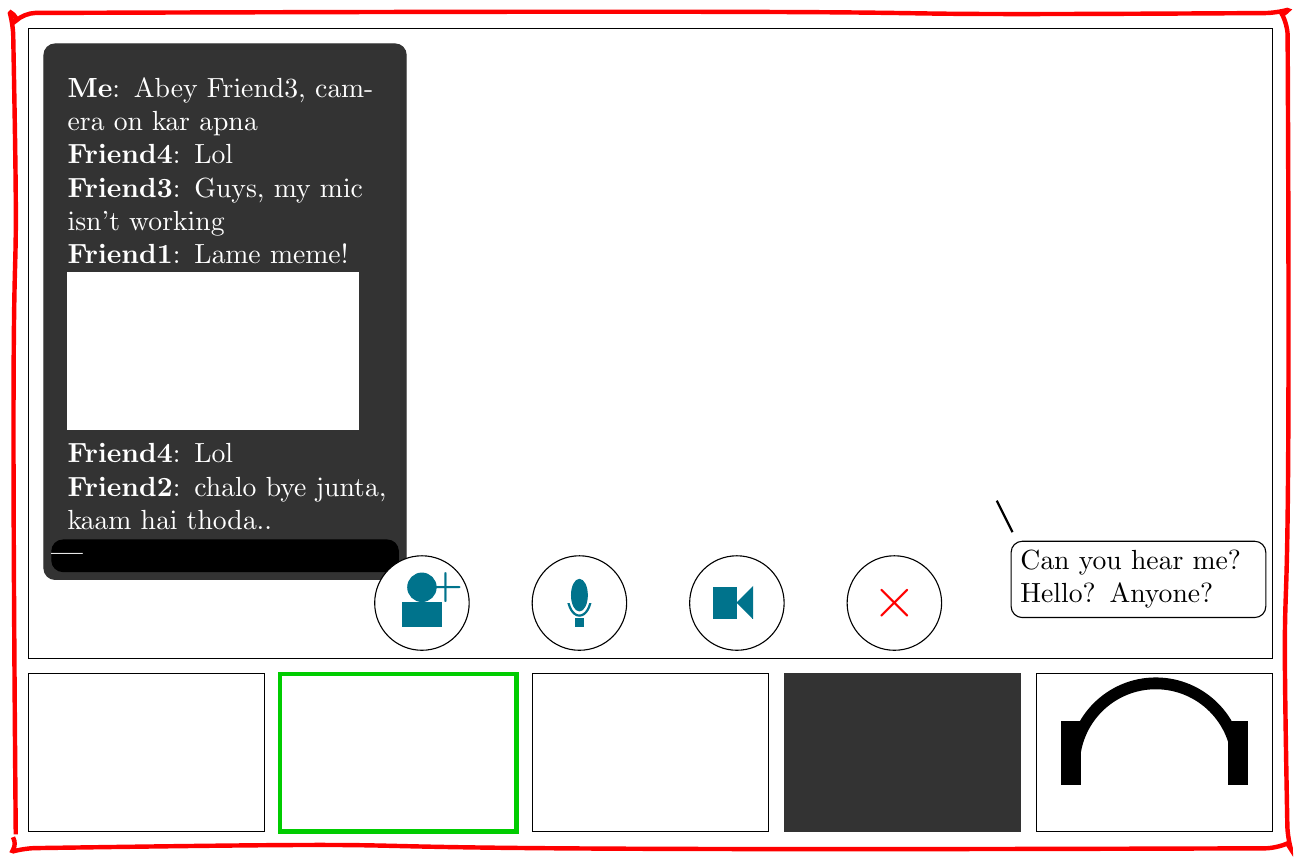
\begin{tikzpicture}[framed, decoration=penciline, background rectangle/.style={ultra thick,draw=red, rounded corners, decorate}]
		\begin{scope}[scale=3.2]
			\clip(0, 0) rectangle (4.5,2.5);
			\newdummy[tshirt=white!40!red, pant=blue!40!green, boyhair, speak]{xshift=1.4cm, yshift=-0.7cm}
		\end{scope}
		\begin{scope}[scale=1.3]
		\clip(0, -0.16) rectangle (2.3,-1.69);
		\newdummy[tshirt=white, tomhair, poker, pupil=yellow]{xshift=-0.3cm, yshift=-2.8cm}
		\end{scope}
		\begin{scope}[scale=0.8]
			\clip(4, -0.25) rectangle (7.75,-2.75);
			\newdummy[tshirt=white!40!red, boyhair, speak]{xshift=4.3cm, yshift=-3.5cm}
		\end{scope}
		\begin{scope}[scale=0.8]
		\clip(8, -0.25) rectangle (11.75,-2.75);
		\newdummy[tshirt=green!70!black, girlhair, normal, pupil=pink]{xshift=8.4cm, yshift=-3.5cm}
		\end{scope}
		\begin{scope}[scale=0.8]
		\clip(16, -0.25) rectangle (19.75,-2.75);
		\newdummy[tshirt=blue!40!red, tomhair, smile, hair=brown!30!black, pupil=green]{xshift=16.4cm, yshift=-3.5cm}
		\filldraw[] (16.4, -1) rectangle (16.7, -2);
		\filldraw[] (19.05, -1) rectangle (19.35, -2);
		\clip (16.04,-1.5) rectangle (19.35, 0);
		\draw[line width=1.5mm] (17.9,-1.7) circle(1.3);
		\end{scope}
		\draw[](0,0) rectangle (15.8,8);
		\node[rectangle,fill= white, rounded corners, draw, text width=3cm] at (14.1, 1) {Can you hear me? Hello? Anyone?};
		\draw[black, thick] (12.3, 2) -- (12.5, 1.6);
		\filldraw[black!80!white, rounded corners] (0.2, 1) rectangle (4.8, 7.8);
		\filldraw[white] (0.5, 2.9) rectangle (4.2,4.9);
		\filldraw[black, rounded corners] (0.3, 1.1) rectangle (4.7, 1.5);
		\node[white, font=\fontsize{10}{10}] at (0.5, 1.3) {\textbf{|}};
		\node[white, font=\fontsize{10}{10}, align=left, text width=4.2cm] at (2.6, 4.5){\textbf{Me}: Abey Friend3, camera on kar apna\\  \textbf{Friend4}: Lol \\\textbf{Friend3}: Guys, my mic isn't working \\\textbf{Friend1}: Lame meme!\\a\\a\\a\\a\\a\\ \textbf{Friend4}: Lol\\\textbf{Friend2}: chalo bye junta, kaam hai thoda..};
		\draw[](0,-0.2) rectangle (3,-2.2);
		\draw[ultra thick, green!80!black](3.2,-0.2) rectangle (6.2,-2.2);
		\draw[](6.4,-0.2) rectangle (9.4,-2.2);
		\filldraw[black!80!white](9.6,-0.2) rectangle (12.6,-2.2);
		\draw[](12.8,-0.2) rectangle (15.8,-2.2);
		\filldraw[white, draw=black] (5, 0.7) circle (0.6);
		\filldraw[white, draw=black] (7, 0.7) circle (0.6);
		\filldraw[white, draw=black] (9, 0.7) circle (0.6);
		\filldraw[white, draw=black] (11, 0.7) circle (0.6);
		\filldraw[blue!55!green] (4.75, 0.7) rectangle (5.25, 0.4);
		\filldraw[blue!55!green] (5, 0.9) circle (0.18);
		\node[blue!55!green, font=\fontsize{15}{15}] at (5.3, 0.9) {\textbf{+}};
		\filldraw[blue!55!green] (8.7, 0.9) rectangle (9, 0.5);
		\filldraw[blue!55!green] (9, 0.7) -- (9.2, 0.9) -- (9.2, 0.5);
		\node[red, font=\fontsize{20}{20}] at (11, 0.7) {\textbf{$\times$}};
		\filldraw[blue!55!green] (6.95, 0.5) rectangle (7.05, 0.4);
		\filldraw[blue!55!green] (7, 0.8) ellipse (1mm and 2mm);
		\clip (6.5,0.7) rectangle (7.5, 0.2);
		\draw[thick, blue!55!green] (7, 0.8) ellipse (1.5mm and 2.6mm);
	\end{tikzpicture}
\end{comics}

\end{document}